\documentclass[11pt,a4paper]{article}

% ---------- Język i kodowanie ----------
\usepackage{iftex}
\ifPDFTeX                      % pdfLaTeX (m.in. domyslny silnik Overleafa)
  \usepackage[T1]{fontenc}
  \usepackage[utf8]{inputenc}
  \usepackage{lmodern}
\else                          % XeLaTeX / LuaLaTeX / Tectonic
  \usepackage{fontspec}
  \setmainfont{lmroman10-regular.otf}[
    BoldFont=lmroman10-bold.otf, ItalicFont=lmroman10-italic.otf,
    BoldItalicFont=lmroman10-bolditalic.otf]
  \setmonofont{lmmono10-regular.otf}
\fi
\usepackage[polish]{babel}

% ---------- Matematyka, grafika, tabele ----------
\usepackage{amsmath}
\usepackage{amssymb}
\usepackage{graphicx}
\usepackage{booktabs}
\usepackage{float}
\usepackage{caption}
\usepackage{multirow}
\usepackage[margin=2.5cm]{geometry}
\usepackage{pgfplots}
\pgfplotsset{compat=1.18}
\pgfplotsset{
  wykres/.style={
    width=0.92\textwidth, height=7cm, grid=both,
    grid style={line width=0.2pt, draw=gray!25},
    major grid style={line width=0.4pt, draw=gray!45},
    xlabel={Częstotliwość $f$ [MHz]},
    legend pos=north west, legend cell align=left, legend columns=2,
    legend style={font=\footnotesize, fill=white, draw=gray!50,
                  /tikz/every even column/.append style={column sep=1.2em}},
    enlarge y limits={upper, value=0.32},   % zapas u gory pod legende
    title style={font=\small, yshift=0.2em},
    unbounded coords=jump, tick label style={font=\footnotesize}
  }
}
\usepackage[hidelinks,unicode]{hyperref}
\emergencystretch=1em

% Suma impedancji układu dopasowującego: Zg + ZL = 50 + 50 Ohm.
\newcommand{\Zsum}{100\ \Omega}

\title{\textbf{Pomiar tłumienności materiałów absorpcyjnych}\\[0.3em]
\large Laboratorium Kompatybilności Elektromagnetycznej\\
i Bezpieczeństwa Elektromagnetycznego --- ćwiczenie nr 5}
\author{% TUTAJ WSTAW IMIONA I NAZWISKA CZŁONKÓW ZESPOŁU
Imię Nazwisko, Imię Nazwisko\\
\small Politechnika Wrocławska, Katedra Telekomunikacji i Teleinformatyki}
\date{Data wykonania ćwiczenia: 12.10.2026\\ \small Prowadzący: % TUTAJ WSTAW PROWADZĄCEGO
}

\begin{document}
\maketitle

\section{Cel ćwiczenia}

Celem ćwiczenia było praktyczne zapoznanie się z techniką pomiaru tłumienności
materiałów absorpcyjnych, doskonalenie umiejętności posługiwania się aparaturą
pomiarową oraz zestawiania toru pomiarowego, a także wyznaczenie impedancji
badanych elementów na podstawie zmierzonej tłumienności w zadanym układzie
pomiarowym. Badaniu poddano dwa rdzenie ferrytowe Würth Elektronik
z~serii WE-AFB o~numerach katalogowych \textbf{74270043} oraz \textbf{74270044},
każdy w~konfiguracji z~pojedynczym i~podwójnym uzwojeniem.

\section{Stanowisko pomiarowe}

\subsection{Informacje wstępne}

Pomiary wykonano podczas zajęć laboratoryjnych w~sali 347 budynku C-4
Politechniki Wrocławskiej.

\subsection{Metoda pomiarowa}

Zastosowano metodę pomiaru tłumienności wtrąceniowej w~torze o~znanej impedancji.
Badany element montowano bezpośrednio na „żyle gorącej” układu dopasowującego,
zapewniającego dopasowanie impedancyjne toru. Jako źródło sygnału wykorzystano
generator śledzący (\emph{tracking generator}) analizatora widma, a~poziom sygnału
odczytywano na tym samym analizatorze.

Czynności przygotowawcze --- stabilizację układu na płycie wsporczej, kontrolę
sprzężenia pojemnościowego, zachowanie stałej odległości zacisków adapterów oraz
prostopadłe prowadzenie przewodów współosiowych --- wykonano zgodnie z~instrukcją
do ćwiczenia.

\subsection{Konfiguracja stanowiska pomiarowego}

\subsubsection{Spis aparatury pomiarowej}
\begin{itemize}
  \item analizator widma z~generatorem śledzącym (odbiornik EMC, oprogramowanie HMExplorer),
  \item układ dopasowujący z~płytą wsporczą,
  \item adaptery dopasowujące ($50\ \Omega$),
  \item przewody współosiowe,
  \item żyły (przewody pojedyncze) o~różnych długościach,
  \item rdzenie ferrytowe Würth Elektronik 74270043 i~74270044 (w~wersji z~pojedynczym
        oraz fabrycznie przygotowanym podwójnym uzwojeniem).
\end{itemize}

\subsubsection{Opis konfiguracji}

Analizator z~włączonym generatorem śledzącym podłączono do adapterów zamontowanych
na płycie wsporczej. Pomiędzy adaptery wpinano przewód (żyłę pojedynczą) o~długości
dobranej do rozmiaru badanego rdzenia, tak aby odległość między adapterami pozostawała
identyczna dla pomiaru referencyjnego i~pomiaru z~danym typem ferrytu. Montaż przewodu
oraz przekładanie adapterów wykonano zgodnie z~instrukcją.

\begin{figure}[H]
  \centering
  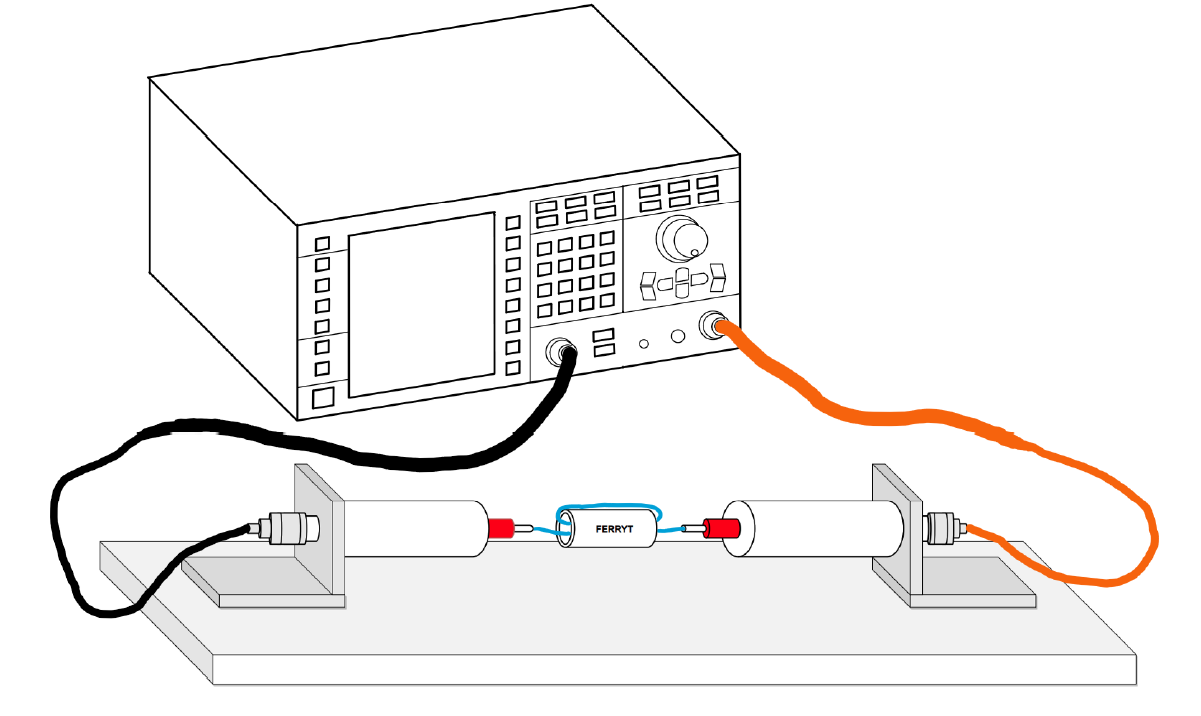
\includegraphics[width=0.85\textwidth]{rys_stanowisko.png}
  \caption{Ogólny schemat stanowiska do wyznaczania tłumienności badanych elementów
           (wg Rys.~2-1 z~instrukcji do ćwiczenia).}
  \label{fig:stanowisko}
\end{figure}

\section{Realizacja ćwiczenia}

\subsection{Pomiar referencyjny}

Układ zestawiono zgodnie ze schematem (rys.~\ref{fig:stanowisko}), bez badanego
elementu --- mierzono poziom sygnału przenoszonego przez sam przewód. Na analizatorze
widma ustawiono parametry zebrane w~tabeli~\ref{tab:param-reczny}.

\begin{table}[H]
  \centering
  \caption{Nastawy analizatora widma dla pomiaru metodą ręczną (z użyciem markera).}
  \label{tab:param-reczny}
  \begin{tabular}{ll}
    \toprule
    \textbf{Parametr} & \textbf{Wartość} \\
    \midrule
    Mode                & sweep \\
    Tracking generator  & ON \\
    Zakres częstotliwości & $1\ \mathrm{MHz} - 1000\ \mathrm{MHz}$ \\
    RBW                 & $100\ \mathrm{kHz}$ \\
    Jednostki           & $\mathrm{dB\mu V}$ \\
    Detektor            & Max peak \\
    \bottomrule
  \end{tabular}
\end{table}

Pomiar wykonano przy użyciu markera, rejestrując poziom sygnału w~40 punktach
częstotliwościowych. Krok częstotliwości dobierano na bieżąco --- gęściej w~obszarach
szybkich zmian przebiegu, rzadziej tam, gdzie charakterystyka zmieniała się wolno.

\subsection{Pomiar poziomu sygnału z~zamontowanym badanym elementem}

Pomiary z~badanym elementem przeprowadzono przy niezmienionych nastawach analizatora
oraz niezmienionej geometrii układu. Rdzeń instalowano centrycznie na przewodzie,
pomiędzy adapterami dopasowującymi, a~odczyty wykonywano dokładnie na tych samych
częstotliwościach co w~pomiarze referencyjnym. Metodą ręczną zbadano rdzeń
\textbf{74270043} w~konfiguracji z~pojedynczym oraz podwójnym uzwojeniem
(rdzenie z~podwójnym uzwojeniem były przygotowane fabrycznie na stanowisku).

\subsection{Pomiar metodą automatyczną}

Pomiar automatyczny wykonano w~programie HMExplorer (tryb \emph{EMC PreCom})
zgodnie z~instrukcją dodatkową do ćwiczenia; nastawy zestawiono
w~tabeli~\ref{tab:param-auto}, a~zarejestrowane przebiegi wyeksportowano
do plików CSV.

\begin{table}[H]
  \centering
  \caption{Nastawy pomiaru automatycznego (HMExplorer, EMC PreCom).}
  \label{tab:param-auto}
  \begin{tabular}{ll}
    \toprule
    \textbf{Parametr} & \textbf{Wartość} \\
    \midrule
    Zakres częstotliwości   & $1\ \mathrm{MHz} - 1000\ \mathrm{MHz}$ \\
    Stepsize                & $1\ \mathrm{MHz}$ \\
    Measure time            & $50\ \mathrm{ms}$ \\
    Reference level         & domyślny \\
    RBW (Premeasure)        & $100\ \mathrm{kHz}$ \\
    RBW (Final measure)     & domyślny \\
    Preamplifier            & OFF \\
    Tracking generator      & ON \\
    \bottomrule
  \end{tabular}
\end{table}

\begin{figure}[H]
  \centering
  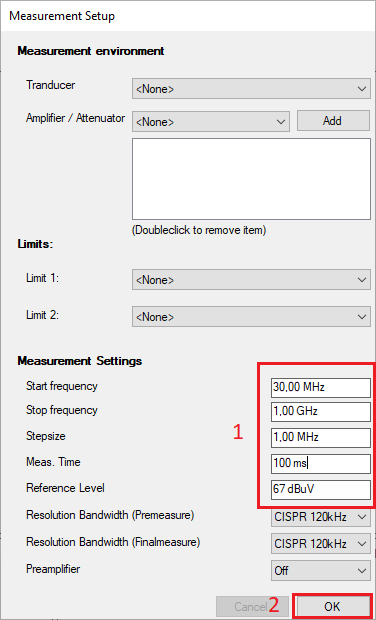
\includegraphics[width=0.30\textwidth]{rys_precom_setup.png}
  \caption{Okno \emph{Measurement Setup} programu HM PreCom EMC, w~którym wprowadzono
           parametry pomiaru. Zrzut pochodzi z~instrukcji i~ma charakter poglądowy ---
           wartości zastosowane w~ćwiczeniu zestawiono w~tabeli~\ref{tab:param-auto}.}
  \label{fig:precom}
\end{figure}

Metodą automatyczną zarejestrowano cztery przebiegi po 1000 punktów każdy ---
rdzeń 74270043 oraz 74270044, w~konfiguracji z~pojedynczym i~podwójnym uzwojeniem ---
w~plikach:
\begin{itemize}
  \item \texttt{pojedynczy\_74270043.csv}, \texttt{podwojny\_74270043.csv},
  \item \texttt{pojedynczy\_74270044.csv}, \texttt{podwojny\_74270044.csv}.
\end{itemize}

\subsection{Wyznaczenie tłumienności badanych elementów}

Tłumienność badanego elementu wyznaczono jako różnicę poziomów sygnału zmierzonych
w~układzie referencyjnym i~w~układzie z~zamontowanym rdzeniem:
\begin{equation}
A\,[\mathrm{dB}] = \left| U_2\,[\mathrm{dB\mu V}] - U_1\,[\mathrm{dB\mu V}] \right|,
\label{eq:tlumiennosc}
\end{equation}
gdzie $U_1$ --- napięcie zmierzone w~układzie referencyjnym (sam przewód),
$U_2$ --- napięcie w~układzie z~badanym elementem. W~tabelach podano wartości
ze znakiem, tj. $A = U_1 - U_2$: wartości dodatnie oznaczają rzeczywiste tłumienie
wnoszone przez rdzeń, natomiast nieliczne wartości ujemne (poziom w~układzie
z~ferrytem wyższy niż w~układzie referencyjnym) są skutkiem niepewności pomiaru
oraz zjawisk rezonansowych w~torze, a~nie wzmocnienia sygnału --- dla takich punktów
impedancji nie wyznaczano (oznaczenie „---” w~tabelach).

\paragraph{Uwaga metodyczna.} Dla pomiaru automatycznego nie zarejestrowano
osobnego przebiegu referencyjnego. Jako referencję dla danych z~plików CSV przyjęto
charakterystykę referencyjną z~pomiaru ręcznego, interpolowaną liniowo na siatkę
częstotliwości o~kroku $1\ \mathrm{MHz}$. Założenie to jest uprawnione, ponieważ
oba pomiary wykonano w~tym samym torze i~przy tej samej geometrii układu, jednak
wnosi ono dodatkową niepewność, szczególnie w~zakresie powyżej $300\ \mathrm{MHz}$,
gdzie charakterystyka referencyjna wykazuje silne falowanie.

\subsection{Obliczenie impedancji badanych elementów}

Impedancję badanego elementu wyznaczono z~zmierzonej tłumienności:
\begin{equation}
Z_B = \left( 10^{\frac{A}{20}} - 1 \right)\left( Z_g + Z_L \right),
\label{eq:impedancja}
\end{equation}
gdzie $Z_g$ i~$Z_L$ to impedancje układu dopasowującego. Obliczenia wykonano, przyjmując
$Z_g = Z_L = 50\ \Omega$, czyli $Z_g + Z_L = \Zsum$. Przykładowo dla rdzenia
74270043 z~podwójnym uzwojeniem przy $f = 55{,}94\ \mathrm{MHz}$
($A = 15{,}96\ \mathrm{dB}$):
\begin{equation}
Z_B = \left( 10^{\frac{15{,}96}{20}} - 1 \right) \cdot 100\ \Omega
    = \left( 6{,}28 - 1 \right) \cdot 100\ \Omega \approx 528\ \Omega .
\end{equation}
Przy ocenie wyników dla podwójnego uzwojenia wykorzystano zależność impedancji
rdzenia od liczby zwojów $N$:
\begin{equation}
Z_B(N) \approx N^2 \, Z_B(1),
\label{eq:n2}
\end{equation}
zgodnie z~którą podwojenie liczby zwojów powinno czterokrotnie zwiększyć impedancję.

\section{Opracowanie wyników}

\subsection{Wyniki pomiaru metodą ręczną}

\begin{table}[H]
  \centering
  \small
  \caption{Pomiar ręczny: poziomy sygnału, tłumienność i~impedancja rdzenia 74270043
           ($Z_g+Z_L = \Zsum$). Indeks „1z” --- pojedyncze uzwojenie, „2z” --- podwójne uzwojenie.}
  \label{tab:reczny}
  \begin{tabular}{rrrrrrrr}
    \toprule
    $f$ & $U_{ref}$ & $U_{1z}$ & $U_{2z}$ & $A_{1z}$ & $A_{2z}$ & $Z_{1z}$ & $Z_{2z}$ \\
    $[\mathrm{MHz}]$ & $[\mathrm{dB\mu V}]$ & $[\mathrm{dB\mu V}]$ & $[\mathrm{dB\mu V}]$
    & $[\mathrm{dB}]$ & $[\mathrm{dB}]$ & $[\Omega]$ & $[\Omega]$ \\
    \midrule
    2.00 & 96.86 & 95.92 & 99.58 & +0.94 & -2.72 & 11 & -- \\
    11.99 & 97.76 & 96.27 & 90.97 & +1.49 & +6.79 & 19 & 119 \\
    33.97 & 97.31 & 91.27 & 82.79 & +6.04 & +14.52 & 100 & 432 \\
    55.94 & 96.70 & 89.62 & 80.74 & +7.08 & +15.96 & 126 & 528 \\
    91.91 & 97.08 & 90.11 & 81.21 & +6.97 & +15.87 & 123 & 522 \\
    127.87 & 95.54 & 88.79 & 79.90 & +6.75 & +15.64 & 118 & 505 \\
    151.85 & 94.28 & 88.21 & 79.72 & +6.07 & +14.56 & 101 & 435 \\
    193.81 & 94.54 & 89.86 & 82.17 & +4.68 & +12.37 & 71 & 315 \\
    223.78 & 92.86 & 88.90 & 81.68 & +3.96 & +11.18 & 58 & 262 \\
    247.75 & 91.64 & 88.71 & 82.18 & +2.93 & +9.46 & 40 & 197 \\
    265.73 & 91.93 & 89.70 & 83.72 & +2.23 & +8.21 & 29 & 157 \\
    293.71 & 92.44 & 90.73 & 85.62 & +1.71 & +6.82 & 22 & 119 \\
    317.68 & 91.12 & 90.06 & 85.67 & +1.06 & +5.45 & 13 & 87 \\
    337.66 & 90.00 & 89.64 & 85.94 & +0.36 & +4.06 & 4 & 60 \\
    361.64 & 90.78 & 90.88 & 88.20 & -0.10 & +2.58 & -- & 35 \\
    389.61 & 91.72 & 92.18 & 90.19 & -0.46 & +1.53 & -- & 19 \\
    413.59 & 90.75 & 91.57 & 90.31 & -0.82 & +0.44 & -- & 5 \\
    429.57 & 90.08 & 91.09 & 90.47 & -1.01 & -0.39 & -- & -- \\
    459.54 & 91.36 & 92.43 & 92.18 & -1.07 & -0.82 & -- & -- \\
    489.51 & 92.95 & 93.74 & 93.29 & -0.79 & -0.34 & -- & -- \\
    507.49 & 92.32 & 93.17 & 92.70 & -0.85 & -0.38 & -- & -- \\
    513.49 & 91.89 & 92.84 & 92.25 & -0.95 & -0.36 & -- & -- \\
    557.44 & 93.73 & 93.17 & 90.72 & +0.56 & +3.01 & 7 & 41 \\
    583.42 & 95.04 & 93.94 & 91.42 & +1.10 & +3.62 & 14 & 52 \\
    615.38 & 93.82 & 91.72 & 88.83 & +2.10 & +4.99 & 27 & 78 \\
    651.35 & 92.78 & 90.38 & 87.74 & +2.40 & +5.04 & 32 & 79 \\
    677.32 & 93.07 & 90.67 & 88.71 & +2.40 & +4.36 & 32 & 65 \\
    707.29 & 90.54 & 88.05 & 86.82 & +2.49 & +3.72 & 33 & 53 \\
    741.26 & 88.53 & 86.02 & 85.67 & +2.51 & +2.86 & 34 & 39 \\
    755.24 & 88.99 & 86.35 & 86.38 & +2.64 & +2.61 & 36 & 35 \\
    773.23 & 89.64 & 86.74 & 87.26 & +2.90 & +2.38 & 40 & 32 \\
    799.20 & 87.90 & 84.61 & 85.55 & +3.29 & +2.35 & 46 & 31 \\
    829.17 & 86.45 & 82.86 & 84.10 & +3.59 & +2.35 & 51 & 31 \\
    851.15 & 85.17 & 83.52 & 85.11 & +1.65 & +0.06 & 21 & 1 \\
    873.13 & 88.75 & 84.04 & 86.12 & +4.71 & +2.63 & 72 & 35 \\
    893.11 & 87.85 & 82.72 & 84.99 & +5.13 & +2.86 & 81 & 39 \\
    915.08 & 87.16 & 81.52 & 83.95 & +5.64 & +3.21 & 91 & 45 \\
    943.06 & 88.81 & 82.05 & 85.03 & +6.76 & +3.78 & 118 & 55 \\
    969.03 & 90.49 & 83.27 & 85.61 & +7.22 & +4.88 & 130 & 75 \\
    1000.00 & 89.57 & 81.95 & 85.11 & +7.62 & +4.46 & 140 & 67 \\
    \bottomrule
  \end{tabular}
\end{table}

\begin{figure}[H]
  \centering
  \begin{tikzpicture}
    \begin{axis}[wykres, xmode=log, ylabel={Tłumienność $A$ [dB]},
                 title={Tłumienność rdzenia 74270043 --- pomiar ręczny}]
      \addplot[thick, mark=*, mark size=1.2pt] table[x=f, y=A1z] {dane_reczny.dat};
      \addlegendentry{74270043 --- 1 zwój}
      \addplot[thick, dashed, mark=square*, mark size=1.2pt] table[x=f, y=A2z] {dane_reczny.dat};
      \addlegendentry{74270043 --- 2 zwoje}
      \draw[gray, dotted] (axis cs:1,0) -- (axis cs:1000,0);
    \end{axis}
  \end{tikzpicture}
  \caption{Tłumienność rdzenia 74270043 w~funkcji częstotliwości --- pomiar ręczny
           (skala logarytmiczna na osi częstotliwości).}
  \label{fig:reczny-A}
\end{figure}

\begin{figure}[H]
  \centering
  \begin{tikzpicture}
    \begin{axis}[wykres, xmode=log, ymode=log, ylabel={Impedancja $Z_B$ [$\Omega$]},
                 title={Impedancja rdzenia 74270043 --- pomiar ręczny}]
      \addplot[thick, mark=*, mark size=1.2pt] table[x=f, y=Z1z] {dane_reczny.dat};
      \addlegendentry{74270043 --- 1 zwój}
      \addplot[thick, dashed, mark=square*, mark size=1.2pt] table[x=f, y=Z2z] {dane_reczny.dat};
      \addlegendentry{74270043 --- 2 zwoje}
    \end{axis}
  \end{tikzpicture}
  \caption{Impedancja rdzenia 74270043 w~funkcji częstotliwości --- pomiar ręczny
           (skala log--log). Punkty o~ujemnej tłumienności pominięto.}
  \label{fig:reczny-Z}
\end{figure}

\subsection{Wyniki pomiaru metodą automatyczną}

Tabele~\ref{tab:auto-A} i~\ref{tab:auto-Z} zawierają wartości dla wybranych
częstotliwości; pełne przebiegi (1000 punktów na serię) przedstawiono na
wykresach~\ref{fig:auto-A} i~\ref{fig:auto-Z}.

\begin{table}[H]
  \centering
  \small
  \caption{Pomiar automatyczny: tłumienność $A$ wyznaczona względem interpolowanej
           charakterystyki referencyjnej.}
  \label{tab:auto-A}
  \begin{tabular}{rrrrrr}
    \toprule
    \multirow{2}{*}{$f$ [MHz]} & \multirow{2}{*}{$U_{ref}$ [dB$\mu$V]}
    & \multicolumn{2}{c}{74270043 --- $A$ [dB]} & \multicolumn{2}{c}{74270044 --- $A$ [dB]} \\
    \cmidrule(lr){3-4}\cmidrule(lr){5-6}
     & & 1 zwój & 2 zwoje & 1 zwój & 2 zwoje \\
    \midrule
    1 & 96.86 & +2.12 & +2.29 & +2.19 & +3.29 \\
    2 & 96.86 & +1.26 & +1.79 & +1.52 & +5.09 \\
    5 & 97.13 & +0.52 & +2.81 & +2.86 & +10.31 \\
    10 & 97.58 & +0.92 & +5.90 & +4.99 & +13.40 \\
    15 & 97.70 & +2.36 & +8.94 & +6.56 & +15.41 \\
    20 & 97.60 & +3.71 & +11.15 & +7.71 & +16.92 \\
    30 & 97.39 & +5.68 & +13.94 & +9.27 & +18.64 \\
    50 & 96.86 & +7.19 & +15.91 & +10.37 & +19.90 \\
    70 & 96.85 & +7.10 & +15.96 & +10.06 & +19.68 \\
    100 & 96.73 & +6.78 & +15.51 & +9.37 & +18.88 \\
    150 & 94.38 & +6.08 & +14.72 & +8.45 & +17.56 \\
    200 & 94.19 & +3.93 & +12.01 & +5.97 & +14.23 \\
    300 & 92.09 & +0.51 & +6.35 & +2.05 & +5.81 \\
    400 & 91.30 & -2.14 & +0.88 & -0.84 & -2.00 \\
    500 & 92.58 & -1.95 & -0.41 & -0.07 & +1.44 \\
    600 & 94.41 & +0.59 & +4.57 & +3.71 & +6.53 \\
    700 & 91.16 & -0.65 & +4.08 & +3.15 & +5.69 \\
    800 & 87.86 & -0.77 & +2.66 & +2.86 & +4.62 \\
    900 & 87.63 & +1.24 & +3.23 & +4.80 & +6.52 \\
    1000 & 89.57 & +3.47 & +4.67 & +7.68 & +20.64 \\
    \bottomrule
  \end{tabular}
\end{table}

\begin{table}[H]
  \centering
  \small
  \caption{Pomiar automatyczny: impedancja $Z_B$ wyznaczona ze wzoru~\eqref{eq:impedancja}
           dla $Z_g+Z_L=\Zsum$.}
  \label{tab:auto-Z}
  \begin{tabular}{rrrrr}
    \toprule
    \multirow{2}{*}{$f$ [MHz]} & \multicolumn{2}{c}{74270043 --- $Z_B$ [$\Omega$]}
    & \multicolumn{2}{c}{74270044 --- $Z_B$ [$\Omega$]} \\
    \cmidrule(lr){2-3}\cmidrule(lr){4-5}
     & 1 zwój & 2 zwoje & 1 zwój & 2 zwoje \\
    \midrule
    1 & 28 & 30 & 29 & 46 \\
    2 & 16 & 23 & 19 & 80 \\
    5 & 6 & 38 & 39 & 228 \\
    10 & 11 & 97 & 78 & 368 \\
    15 & 31 & 180 & 113 & 489 \\
    20 & 53 & 261 & 143 & 601 \\
    30 & 92 & 398 & 191 & 755 \\
    50 & 129 & 525 & 230 & 889 \\
    70 & 126 & 528 & 218 & 864 \\
    100 & 118 & 497 & 194 & 779 \\
    150 & 101 & 444 & 164 & 655 \\
    200 & 57 & 299 & 99 & 415 \\
    300 & 6 & 108 & 27 & 95 \\
    400 & -- & 11 & -- & -- \\
    500 & -- & -- & -- & 18 \\
    600 & 7 & 69 & 53 & 112 \\
    700 & -- & 60 & 44 & 92 \\
    800 & -- & 36 & 39 & 70 \\
    900 & 15 & 45 & 74 & 112 \\
    1000 & 49 & 71 & 142 & 976 \\
    \bottomrule
  \end{tabular}
\end{table}

\begin{figure}[H]
  \centering
  \begin{tikzpicture}
    \begin{axis}[wykres, xmode=log, ylabel={Tłumienność $A$ [dB]},
                 title={Tłumienność badanych rdzeni --- pomiar automatyczny}]
      \addplot[thick] table[x=f, y=A43p] {dane_auto.dat}; \addlegendentry{74270043 --- 1 zwój}
      \addplot[thick, dashed] table[x=f, y=A43d] {dane_auto.dat}; \addlegendentry{74270043 --- 2 zwoje}
      \addplot[thick, densely dotted] table[x=f, y=A44p] {dane_auto.dat}; \addlegendentry{74270044 --- 1 zwój}
      \addplot[thick, dashdotted] table[x=f, y=A44d] {dane_auto.dat}; \addlegendentry{74270044 --- 2 zwoje}
      \draw[gray, dotted] (axis cs:1,0) -- (axis cs:1000,0);
    \end{axis}
  \end{tikzpicture}
  \caption{Tłumienność badanych rdzeni --- pomiar automatyczny, krok $1\ \mathrm{MHz}$.}
  \label{fig:auto-A}
\end{figure}

\begin{figure}[H]
  \centering
  \begin{tikzpicture}
    \begin{axis}[wykres, xmode=log, ymode=log, ylabel={Impedancja $Z_B$ [$\Omega$]},
                 title={Impedancja badanych rdzeni --- pomiar automatyczny}]
      \addplot[thick] table[x=f, y=Z43p] {dane_auto.dat}; \addlegendentry{74270043 --- 1 zwój}
      \addplot[thick, dashed] table[x=f, y=Z43d] {dane_auto.dat}; \addlegendentry{74270043 --- 2 zwoje}
      \addplot[thick, densely dotted] table[x=f, y=Z44p] {dane_auto.dat}; \addlegendentry{74270044 --- 1 zwój}
      \addplot[thick, dashdotted] table[x=f, y=Z44d] {dane_auto.dat}; \addlegendentry{74270044 --- 2 zwoje}
    \end{axis}
  \end{tikzpicture}
  \caption{Impedancja badanych rdzeni --- pomiar automatyczny (skala log--log).
           Przedziały, w~których wyznaczona tłumienność była ujemna, stanowią przerwy w~przebiegu.}
  \label{fig:auto-Z}
\end{figure}

\subsection{Zestawienie wartości charakterystycznych}

\begin{table}[H]
  \centering
  \small
  \caption{Maksymalna tłumienność i~odpowiadająca jej impedancja (pomiar automatyczny).}
  \label{tab:maksima}
  \begin{tabular}{llrrr}
    \toprule
    Rdzeń & Konfiguracja & $A_{max}$ [dB] & $f(A_{max})$ [MHz] & $Z_B(A_{max})$ [$\Omega$] \\
    \midrule
    74270043 & 1 zwój  & 7.23  & 64  & 130 \\
    74270043 & 2 zwoje & 16.07 & 62  & 536 \\
    74270044 & 1 zwój  & 10.41 & 49  & 232 \\
    74270044 & 2 zwoje & 19.97 & 53  & 897 \\
    \bottomrule
  \end{tabular}
\end{table}

Maksima wyznaczono w~paśmie do $300\ \mathrm{MHz}$. Powyżej tej granicy przebiegi
zaburzają rezonanse toru pomiarowego: dla rdzenia 74270044 z~podwójnym uzwojeniem
formalnie największą wartość, $20{,}6\ \mathrm{dB}$, zarejestrowano przy
$999\ \mathrm{MHz}$, lecz jest to artefakt na skraju zakresu, a~nie maksimum
charakterystyki absorpcyjnej, dlatego wartości tej nie uwzględniono.

\subsection{Porównanie z~notami katalogowymi}

Badane elementy należą do rodziny Würth Elektronik WE-AFB (EMI Suppression Axial
Ferrite Bead); rdzeń 74270043 wykonano z~materiału 3W800, a~74270044 z~materiału
4W620. Dane katalogowe producenta odnoszą się do \emph{jednego zwoju} i~pochodzą
z~pomiaru na odcinku przewodu AWG26 o~długości $100\ \mathrm{mm}$; karty katalogowe
zawierają ponadto przebiegi dla dwóch i~trzech zwojów, co potwierdza wykorzystywaną
tu zależność~\eqref{eq:n2}. Zestawienie wartości katalogowych z~wynikami pomiaru
przedstawia tabela~\ref{tab:katalog}.

\begin{table}[H]
  \centering
  \small
  \caption{Porównanie impedancji zmierzonej (1 zwój) z~wartościami katalogowymi
           Würth Elektronik dla serii WE-AFB.}
  \label{tab:katalog}
  \begin{tabular}{lrrrr}
    \toprule
    Rdzeń & $Z_{kat}$ (25 MHz) & $Z_{pom}$ (25 MHz) & $Z_{kat}$ (100 MHz) & $Z_{pom}$ (100 MHz) \\
          & $[\Omega]$ & $[\Omega]$ & $[\Omega]$ & $[\Omega]$ \\
    \midrule
    74270043 & 146 & 73 & 261 & 118 \\
    74270044 & 293 & 169 & 459 & 194 \\
    \bottomrule
  \end{tabular}
\end{table}

\begin{figure}[H]
  \centering
  \begin{tikzpicture}
    \begin{axis}[wykres, xmode=log, ymode=log, ylabel={Impedancja $Z_B$ [$\Omega$]},
                 title={Impedancja zmierzona a~nota katalogowa (1 zwój)}]
      \addplot[thick] table[x=f, y=Z43p] {dane_auto.dat}; \addlegendentry{74270043 --- pomiar (1 zwój)}
      \addplot[thick, densely dotted] table[x=f, y=Z44p] {dane_auto.dat}; \addlegendentry{74270044 --- pomiar (1 zwój)}
      \addplot[only marks, mark=o, mark size=3pt] coordinates {(25,146) (100,261)};
      \addlegendentry{74270043 --- nota katalogowa}
      \addplot[only marks, mark=square, mark size=3pt] coordinates {(25,293) (100,459)};
      \addlegendentry{74270044 --- nota katalogowa}
    \end{axis}
  \end{tikzpicture}
  \caption{Porównanie zmierzonej impedancji rdzeni (1 zwój) z~wartościami katalogowymi producenta.}
  \label{fig:katalog}
\end{figure}

\paragraph{Podobieństwa.} Zmierzone charakterystyki mają ten sam przebieg
jakościowy co katalogowe: impedancja rośnie od pojedynczych omów przy
$1\ \mathrm{MHz}$ do szerokiego maksimum rzędu kilkudziesięciu megaherców,
po czym maleje. Zachowane jest również uszeregowanie elementów, ponieważ rdzeń
74270044 wykazuje w~całym paśmie impedancję istotnie większą niż 74270043,
co odpowiada relacji wartości katalogowych ($459\ \Omega$ wobec $261\ \Omega$
przy $100\ \mathrm{MHz}$).

\paragraph{Różnice.} Wartości bezwzględne zmierzonej impedancji są około dwukrotnie
niższe od katalogowych ($118\ \Omega$ wobec $261\ \Omega$ oraz $194\ \Omega$ wobec
$459\ \Omega$ przy $100\ \mathrm{MHz}$). Przyczyny rozbieżności są następujące:
\begin{itemize}
  \item inna metodyka pomiaru: producent wyznacza impedancję
        analizatorem impedancji w~ściśle zdefiniowanej oprawie pomiarowej,
        natomiast w~ćwiczeniu mierzy się tłumienność wtrąceniową w~torze
        $50\ \Omega$ i~przelicza ją na impedancję przy założeniu idealnego
        dopasowania $Z_g = Z_L$;
  \item sprzężenie pojemnościowe przez rdzeń i~wzdłuż przewodu
        „bocznikuje” impedancję ferrytu, zaniżając wynik tym silniej,
        im wyższa częstotliwość;
  \item niepewność toru: falowanie charakterystyki referencyjnej
        rzędu $\pm 2\ \mathrm{dB}$ przekłada się bezpośrednio na błąd $A$,
        a~przez zależność wykładniczą~\eqref{eq:impedancja} --- na duży błąd $Z_B$;
  \item tolerancja materiału: parametry ferrytów 3W800 i~4W620 podlegają
        rozrzutowi produkcyjnemu i~zależą od temperatury;
  \item położenie maksimum: w~pomiarze przypada ono na $50-70\ \mathrm{MHz}$,
        podczas gdy dane katalogowe wykazują wzrost impedancji jeszcze pomiędzy
        $25$ a~$100\ \mathrm{MHz}$. Przesunięcie to jest skutkiem pojemności
        rozproszonych toru pomiarowego, które obniżają częstotliwość rezonansu
        własnego badanego elementu.
\end{itemize}

\section{Wnioski}

Wyniki potwierdzają absorpcyjny charakter badanych rdzeni ferrytowych: maksimum
tłumienności przypada na zakres $50-100\ \mathrm{MHz}$ i~wynosi $7{,}2\ \mathrm{dB}$
dla rdzenia 74270043 oraz $10{,}4\ \mathrm{dB}$ dla 74270044 przy pojedynczym
uzwojeniu, podczas gdy poniżej $10\ \mathrm{MHz}$ pojedynczy zwój pozostaje
praktycznie nieskuteczny. Podwojenie liczby zwojów zwiększyło impedancję przy
$100\ \mathrm{MHz}$ około czterokrotnie (stosunek $4{,}2$ dla 74270043 i~$4{,}0$
dla 74270044), co dobrze potwierdza zależność~\eqref{eq:n2} i~przesuwa użyteczny
zakres pracy w~stronę niższych częstotliwości. Obie metody pomiarowe dały zgodne
rezultaty --- maksymalne tłumienności różnią się o~mniej niż $0{,}2\ \mathrm{dB}$ ---
przy czym metoda automatyczna jest nieporównanie wydajniejsza i~ujawnia szczegóły
przebiegu niewidoczne przy 40 punktach pomiaru ręcznego. Zmierzone impedancje są
jednak około dwukrotnie niższe od katalogowych, a~w~zakresie $350-550\ \mathrm{MHz}$
wynik zaburzają rezonanse toru pomiarowego, dlatego zastosowana metoda nadaje się
do porównawczej oceny elementów absorpcyjnych, lecz nie do wyznaczania bezwzględnych
wartości impedancji.

\end{document}
